% Provenance (never printed): lycee terminale S SVT "Les climats de la Terre"
% and the 2019 enseignement scientifique ("Le climat de la Terre": forcing,
% feedbacks, the IPCC assessments, scenarios), union; physical science only,
% as the user ruled (2026-10-22). See sources/outline_sources.md. Pilot
% chapter, 2026-10-22. Every figure about the climate system is an IPCC AR6
% WG1 statement (ledger ipcc:*) or computed from a dataset in
% figdata/grade-12/climate_records.py.
\chapter{Perubahan Iklim: Pengamatan, Penyebab, dan Proyeksi}\label{ch:g12:climate-change}

Tinggi di lereng utara Mauna Loa, sebuah gunung api di tengah Samudra Pasifik,
sekelompok bangunan putih berdiri di atas lava yang gundul, \qty{3397}{m} di
atas permukaan laut. Di atas sana, di atas lapisan udara yang dicemari oleh
pulau di bawahnya dan ribuan kilometer dari kota besar mana pun, udaranya
kira-kira sebersih dan setercampur atmosfer seluruh planet. Sejak Maret 1958,
karbon dioksidanya telah diukur hampir tanpa putus. Rekaman itu bermula sebagai
proyek seorang ahli kimia; kini rekaman itu telah menjadi kurva yang paling
terkenal dalam ilmu kebumian. Bab ini membaca kurva itu dan rekaman-rekaman
iklim yang lain, menjelaskan bagaimana perubahan di udara mengubah \omterm{def:g10:earth-energy-budget:energy-budget}{neraca
energi} planet, bagaimana para ilmuwan memutuskan apa yang menyebabkan pemanasan
yang mereka amati, dan apa yang mereka proyeksikan untuk dekade-dekade
mendatang.
% ledger: noaa:mlo-site, noaa:keeling-1958

\begin{omfigure}
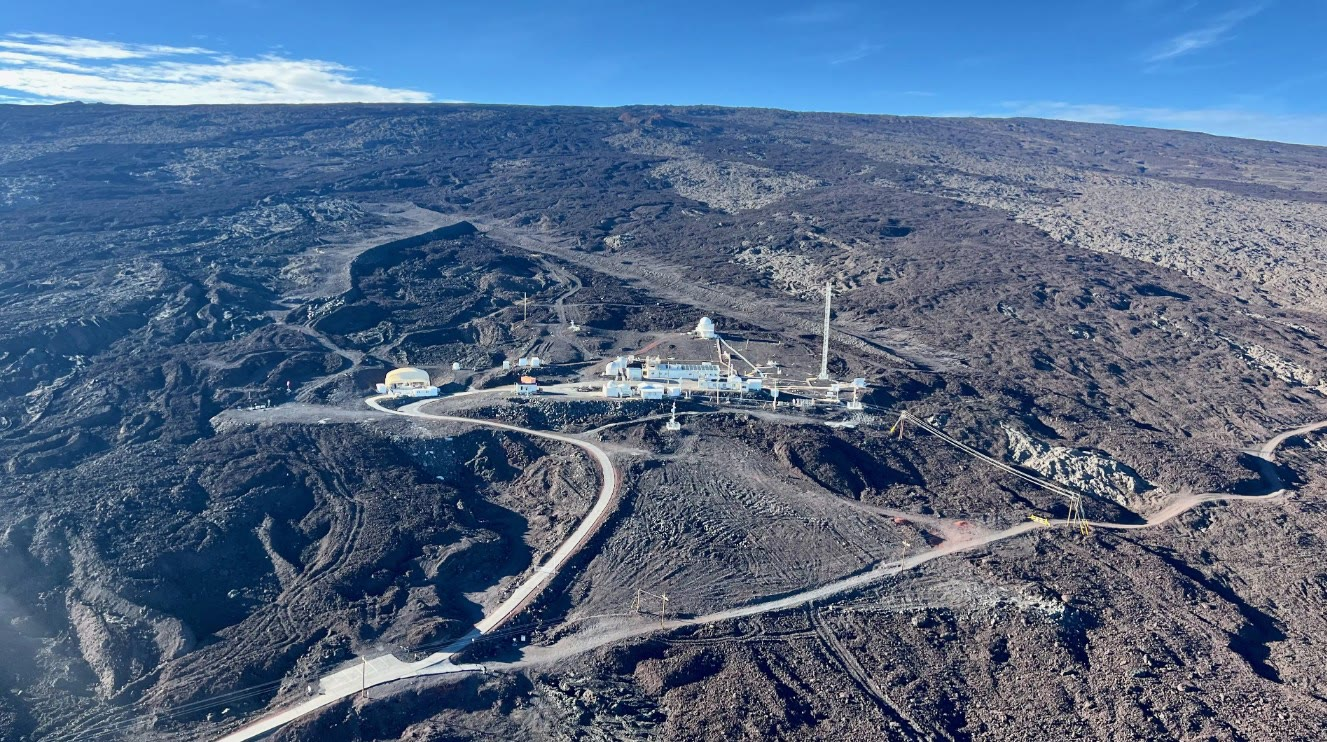
\includegraphics[width=0.78\linewidth]{images/book2/g12-noaa-mauna-loa-observatory.jpg}

{\small Observatorium Mauna Loa, Hawaii, di atas aliran lava tua yang tinggi di
lereng utara gunung api itu. Foto: Brian Vasel, NOAA (domain publik).}
\end{omfigure}

\begin{recall}
Bumi menerima energi dari Matahari sebagai cahaya dan rata-rata kehilangan
jumlah yang sama ke angkasa sebagai radiasi inframerah; bagian sinar Matahari
yang dipantulkan adalah \omterm{def:g10:earth-energy-budget:albedo}{albedo} (\cref{ch:g10:earth-energy-budget}). Gas rumah
kaca --- uap air, karbon dioksida, metana --- menyerap sebagian inframerah yang
dipancarkan permukaan dan mengirim sebagian kembali ke bawah; efek rumah kaca
ini menjaga permukaan jauh lebih hangat daripada seandainya tanpa efek itu
(buku-buku kimia, dan Buku 1, kelas 9). \omterm{def:g12:past-climates:ice-core}{Inti es} menyimpan gelembung udara purba
dan merekam siklus-siklus glasial selama 800\,000 tahun terakhir
(\cref{ch:g12:past-climates}).
\end{recall}

\section{Rekaman-rekaman}

\begin{omfigure}
\begin{tikzpicture}
\begin{axis}[omrecord, width=0.92\linewidth, height=6.2cm, xmin=1957, xmax=2028,
  ymin=305, ymax=440, xlabel={tahun}, ylabel={karbon dioksida (ppm)},
  xtick={1960,1970,...,2020}, /pgf/number format/1000 sep={}]
\addplot[omDef!85!black, line width=0.5pt] table[x=decimal_year, y=co2_ppm] {figdata/out/grade-12-climate_records-co2.dat};
\addplot[only marks, mark=*, mark size=0.9pt, omThm!85!black] table[x=year, y=co2_ppm] {figdata/out/grade-12-climate_records-co2annual.dat};
\end{axis}
\end{tikzpicture}

{\small Kadar karbon dioksida udara di Mauna Loa: rata-rata bulanan (garis)
dan rata-rata tahunan (titik), dalam bagian per juta (ppm) udara kering. Data:
NOAA Global Monitoring Laboratory dan Scripps Institution of Oceanography.}
\end{omfigure}

\begin{proposition}[Rekaman karbon dioksida]\label{prop:g12:climate-change:co2}
% ledger: data:co2-mlo (all numbers computed in figdata/grade-12/climate_records.py)
Di Mauna Loa, konsentrasi karbon dioksida rata-rata tahunan naik dari
\qty{316.0}{ppm} pada 1959 menjadi \qty{427.4}{ppm} pada 2025, dan kenaikannya
makin cepat: konsentrasi itu bertambah sekitar \qty{0.9}{ppm} per tahun pada
dasawarsa 1960-an dan sekitar \qty{2.6}{ppm} per tahun antara 2015 dan 2025.
Setiap tahun konsentrasi itu juga berayun sekitar \qty{7}{ppm}: paling tinggi
pada bulan Mei dan paling rendah pada bulan September.
\end{proposition}

\begin{remark}[Mengapa kurva itu bergerigi]\label{rem:g12:climate-change:teeth}
Ayunan tahunan itu adalah napas vegetasi Belahan Bumi Utara, tempat sebagian
besar tumbuhan darat berada. Pada musim semi dan musim panas, tumbuhan menyerap
lebih banyak karbon dioksida melalui fotosintesis daripada yang dilepaskan oleh
tumbuhan itu sendiri dan tanah; pada musim gugur dan musim dingin, pembusukan
dan respirasi yang menang. Kenaikan dari tahun ke tahun adalah cerita yang
lain: itulah karbon bahan bakar fosil dan hutan yang dibuka, yang menumpuk di
udara.
\end{remark}

\begin{proposition}[Lebih tinggi daripada setidaknya selama dua juta tahun]\label{prop:g12:climate-change:icecore}
% ledger: data:co2-bereiter (173.7 and 298.6 ppm computed), ipcc:co2-2myr (high confidence)
Selama 800\,000 tahun terakhir, gelembung udara es Antarktika merekam
konsentrasi karbon dioksida antara sekitar \qty{174}{ppm}, pada \omterm{def:g12:past-climates:glacial-cycle}{periode glasial}
yang paling dingin, dan \qty{299}{ppm}, pada \omterm{def:g12:past-climates:glacial-cycle}{interglasial} yang paling hangat.
Nilai sekarang terletak lebih dari \qty{100}{ppm} di atas nilai tertinggi itu.
Penilaian-penilaian menyatakan bahwa konsentrasi pada 2019 lebih tinggi
daripada kapan pun dalam setidaknya dua juta tahun (\emph{keyakinan tinggi}).
\end{proposition}

\begin{omfigure}
\begin{tikzpicture}
\begin{axis}[omrecord, omage, width=0.92\linewidth, height=5.2cm, xmin=0, xmax=810,
  ymin=150, ymax=490, xlabel={ribuan tahun sebelum 1950},
  ylabel={karbon dioksida (ppm)}, xtick={0,100,...,800}]
\addplot[omDef!85!black, line width=0.6pt] table[x=age_kyr, y=co2_ppm] {figdata/out/grade-12-climate_records-icecore.dat};
\draw[omThm, densely dashed, line width=0.8pt] (axis cs:810,427.35) -- (axis cs:0,427.35);
\node[font=\footnotesize, text=omThm!85!black, anchor=south west] at (axis cs:780,433) {rata-rata tahunan di Mauna Loa pada 2025};
\end{axis}
\end{tikzpicture}

{\small Karbon dioksida dalam es Antarktika selama 800\,000 tahun: siklus-siklus
glasial menggerakkannya antara sekitar 180 dan \qty{300}{ppm}. Paku tipis di
ujung kanan adalah es termuda, yang merekam awal kenaikan sekarang, sampai
tahun 2001. Data: Bereiter dan kawan-kawan (2015), NOAA Paleoclimatology.}
% the youngest sample of the composite: age -51 yr BP (2001), 368.02 ppm (data/derived/co2-icecore.csv)
\end{omfigure}

\begin{omfigure}
\begin{tikzpicture}
\begin{axis}[omrecord, width=0.92\linewidth, height=5.6cm, xmin=1878, xmax=2027,
  ymin=-0.6, ymax=1.45, xlabel={tahun},
  ylabel={anomali suhu (\unit{\degreeCelsius})},
  xtick={1880,1900,...,2020}, /pgf/number format/1000 sep={},
  legend style={at={(0.03,0.96)}, anchor=north west, font=\footnotesize, draw=black!30}]
\addplot[omDef!70, line width=0.5pt, mark=*, mark size=0.6pt] table[x=year, y=anomaly] {figdata/out/grade-12-climate_records-temp.dat};
\addlegendentry{rata-rata tahunan}
\addplot[omThm!85!black, line width=1.3pt, unbounded coords=jump] table[x=year, y=mean11] {figdata/out/grade-12-climate_records-temp.dat};
\addlegendentry{rata-rata 11 tahun}
\end{axis}
\end{tikzpicture}

{\small Suhu permukaan rata-rata global, sebagai selisih dari rata-ratanya
selama 1951--1980. Data: NASA GISS Surface Temperature Analysis (GISTEMP v4).}
\end{omfigure}

\begin{proposition}[Pemanasan global yang teramati]\label{prop:g12:climate-change:warming}
% ledger: ipcc:gsat-2011-2020, ipcc:decades
Setiap dari empat dekade terakhir lebih hangat daripada dekade mana pun
sebelumnya sejak 1850. Suhu permukaan global 2011--2020 \qty{1.09}{\degreeCelsius}
lebih tinggi daripada suhu 1850--1900 (sangat mungkin antara 0.95 dan
\qty{1.20}{\degreeCelsius}), dengan pemanasan yang lebih besar di atas daratan
(\qty{1.59}{\degreeCelsius}) daripada di atas samudra (\qty{0.88}{\degreeCelsius}).
\end{proposition}

\begin{proposition}[Permukaan laut naik makin cepat]\label{prop:g12:climate-change:sea}
% ledger: ipcc:sea-level-obs, data:gmsl-lsa (3.2 mm/yr trend computed)
Permukaan laut rata-rata global naik sekitar \qty{0.20}{m} antara 1901 dan
2018. Lajunya sekitar \qty{1.3}{mm} per tahun dari 1901 sampai 1971,
\qty{1.9}{mm} per tahun dari 1971 sampai 2006, dan \qty{3.7}{mm} per tahun dari
2006 sampai 2018 (\emph{keyakinan tinggi}). Satelit, yang mengukur tinggi
permukaan laut sejak 1993, mendapati rata-rata \qty{3.2}{mm} per tahun selama
1993--2025. Laut naik karena samudra yang menghangat memuai dan karena gletser
serta lapisan es kehilangan es ke dalamnya.
\end{proposition}

\begin{omfigure}
\begin{tikzpicture}
\begin{axis}[omrecord, width=0.86\linewidth, height=5cm, xmin=1992, xmax=2026,
  ymin=-35, ymax=95, xlabel={tahun}, ylabel={permukaan laut (mm)},
  /pgf/number format/1000 sep={}, xtick={1995,2000,...,2025}]
\addplot[omDef!85!black, line width=0.5pt] table[x=decimal_year, y=gmsl_mm] {figdata/out/grade-12-climate_records-sea.dat};
\end{axis}
\end{tikzpicture}

{\small Permukaan laut rata-rata global yang diukur dari angkasa, kira-kira
setiap sepuluh hari (sinyal musiman dihilangkan), terhadap titik nol yang
dipilih sembarang. Data altimetri disediakan oleh NOAA Laboratory for Satellite
Altimetry.}
\end{omfigure}

\begin{dated}{2025}
% ledger: data:co2-mlo, data:gistemp (values read from the datasets as fetched 2026-10-22)
Konsentrasi karbon dioksida rata-rata tahunan di Mauna Loa pada 2025 adalah
\qty{427.35}{ppm}. Dalam rekaman suhu NASA, tahun terhangat sejauh ini adalah
2024, \qty{1.28}{\degreeCelsius} di atas rata-rata 1951--1980.
\end{dated}

\section{Gaya radiatif}

\begin{definition}[Gaya radiatif]\label{def:g12:climate-change:forcing}
Yang disebut \emph{gaya radiatif}\index{gaya radiatif} sebuah perubahan dalam
sistem iklim --- lebih banyak gas rumah kaca, lebih banyak partikel aerosol,
Matahari yang lebih terang --- adalah perubahan yang ditimbulkannya pada aliran
bersih energi yang memasuki sistem iklim di puncak atmosfer, sebelum suhu
permukaan sempat menanggapinya. Gaya radiatif diukur dalam watt per meter
persegi (\unit{W/m^2}) permukaan Bumi. Gaya yang positif membuat planet
memperoleh energi dan menghangat; gaya yang negatif membuatnya kehilangan
energi dan mendingin.
\end{definition}

\begin{remark}[Gaya efektif]\label{rem:g12:climate-change:effective}
Penilaian-penilaian memakai \omterm{def:g12:climate-change:forcing}{gaya radiatif} \emph{efektif}, yang juga
memperhitungkan penyesuaian cepat atmosfer (misalnya awan-awannya) yang terjadi
sebelum permukaan menghangat. Semua \omterm{def:g12:climate-change:forcing}{gaya} dalam bab ini adalah \omterm{def:g12:climate-change:forcing}{gaya} efektif.
\end{remark}

\begin{proposition}[Gaya sejak 1750]\label{prop:g12:climate-change:forcing}
% ledger: ipcc:erf-total, ipcc:erf-agents
Kegiatan manusia telah menghasilkan \omterm{def:g12:climate-change:forcing}{gaya radiatif} total sebesar
\qty{2.72}{W/m^2} pada 2019 dibandingkan dengan 1750 (sangat mungkin antara 1.96
dan \qty{3.48}{W/m^2}). Gas rumah kaca memberikan \omterm{def:g12:climate-change:forcing}{gaya} yang positif, dipimpin
oleh karbon dioksida (\qty{2.16}{W/m^2}); partikel aerosol, yang memantulkan
sinar Matahari dan membuat awan lebih terang, memberikan \omterm{def:g12:climate-change:forcing}{gaya} yang negatif
(seluruhnya sekitar \qty{-1.06}{W/m^2}). Perubahan kecerahan Matahari selama
periode yang sama hanya memberikan \qty{0.01}{W/m^2}.
\end{proposition}

\begin{omfigure}
% ledger: ipcc:erf-agents, ipcc:erf-total (central values and 5-95 % ranges of AR6 Table 7.8)
\begin{tikzpicture}
\begin{axis}[xbar, width=0.8\linewidth, height=7.2cm, xmin=-1.8, xmax=3.7,
  ytick={1,...,10}, yticklabels={total (manusia), Matahari, tata guna lahan,
  aerosol--awan, aerosol--radiasi, ozon, gas terhalogenasi, dinitrogen oksida,
  metana, karbon dioksida}, y tick label style={font=\small},
  tick label style={font=\small}, xlabel={gaya radiatif efektif, 1750--2019 (\unit{W/m^2})},
  label style={font=\small}, bar width=6pt, bar shift=0pt, axis x line=bottom, axis y line=left,
  axis line style={-}, enlarge y limits=0.07, xmajorgrids,
  grid style={gray!22, line width=0.3pt}, extra x ticks={0},
  extra x tick style={grid style={black!60, line width=0.5pt}}]
\addplot[fill=omThm!55, draw=omThm!80!black, error bars/.cd, x dir=both, x explicit,
  error bar style={black!70}] coordinates {
  (2.16,10) += (0.25,0) -= (0.26,0)
  (0.54,9) += (0.11,0) -= (0.11,0)
  (0.21,8) += (0.03,0) -= (0.03,0)
  (0.41,7) += (0.08,0) -= (0.08,0)
  (0.47,6) += (0.24,0) -= (0.23,0)
  (2.72,1) += (0.76,0) -= (0.76,0)
  (0.01,2) += (0.07,0) -= (0.07,0)};
\addplot[fill=omDef!55, draw=omDef!80!black, error bars/.cd, x dir=both, x explicit,
  error bar style={black!70}] coordinates {
  (-0.22,5) += (0.26,0) -= (0.25,0)
  (-0.84,4) += (0.59,0) -= (0.61,0)
  (-0.20,3) += (0.10,0) -= (0.10,0)};
\end{axis}
\end{tikzpicture}

{\small \omterm{def:g12:climate-change:forcing}{Gaya-gaya} radiatif efektif utama dari 1750 sampai 2019, dengan rentang
sangat mungkin masing-masing (garis galat). Nilai: Laporan Penilaian Keenam
IPCC, Kelompok Kerja~I, Tabel 7.8.}
\end{omfigure}

\begin{proposition}[Karbon dioksida: setiap penggandaan menambahkan gaya yang sama]\label{prop:g12:climate-change:log}
% ledger: ipcc:erf-2xco2, ipcc:log-co2
Dengan pendekatan yang baik, \omterm{def:g12:climate-change:forcing}{gaya} karbon dioksida bertambah menurut
\emph{logaritma} konsentrasinya: setiap penggandaan menambahkan \omterm{def:g12:climate-change:forcing}{gaya} yang sama,
$F_{2\times} = \qty{3.93}{W/m^2}$ untuk penggandaan dari konsentrasi tahun
1750, $C_0 = \qty{278}{ppm}$. \omterm{def:g12:climate-change:forcing}{Gaya} untuk konsentrasi $C$ dengan demikian adalah
\[
  F = F_{2\times}\,\frac{\ln (C/C_0)}{\ln 2}.
\]
\end{proposition}

\begin{example}[Menguji hukum itu terhadap penilaian]\label{ex:g12:climate-change:check}
% ledger: ipcc:erf-2xco2, ipcc:erf-agents
Pada 2019 konsentrasinya \qty{410}{ppm}. Hukum itu memberikan
$F = 3.93 \times \ln(410/278)/\ln 2 = 3.93 \times 0.561 \approx
\qty{2.20}{W/m^2}$, berselisih kurang dari 2\,\% dengan \qty{2.16}{W/m^2} yang diberikan
penilaian untuk karbon dioksida selama 1750--2019.
\end{example}

\begin{proposition}[Ke mana energi tambahan itu pergi]\label{prop:g12:climate-change:heating}
% ledger: ipcc:heating
Karena \omterm{def:g12:climate-change:forcing}{gayanya} positif, sistem iklim memperoleh energi: rata-rata sekitar
\qty{0.79}{W/m^2} selama 2006--2018, naik dari \qty{0.50}{W/m^2} selama
1971--2006 (\emph{keyakinan tinggi}). Samudra menyerap 91\,\% energi ini;
daratan 5\,\%, es yang mencair 3\,\%, dan atmosfer hanya 1\,\%.
\end{proposition}

\section{Umpan balik dan sensitivitas iklim}

Ketika permukaan menghangat, permukaan memancarkan lebih banyak energi ke
angkasa, yang cenderung mengembalikan planet ke dalam keseimbangan. Tetapi
pemanasan itu juga mengubah hal-hal lain --- uap air di udara, salju dan es di
tanah, awan --- dan perubahan-perubahan ini pada gilirannya mengubah \omterm{def:g10:earth-energy-budget:energy-budget}{neraca
energi}.

\begin{definition}[Umpan balik iklim]\label{def:g12:climate-change:feedback}
Yang disebut \emph{umpan balik iklim}\index{umpan balik iklim} adalah perubahan
dalam sistem iklim, yang disebabkan oleh perubahan suhu, yang mengubah \omterm{def:g10:earth-energy-budget:energy-budget}{neraca
energi} dan dengan demikian perubahan suhu itu sendiri. \emph{Umpan balik
positif} memperkuat perubahan awalnya; \emph{umpan balik negatif} meredamnya.
\end{definition}

\begin{example}[Tiga umpan balik]\label{ex:g12:climate-change:three}
\begin{itemize}
  \item \textbf{Uap air (positif).} Udara yang lebih hangat menampung lebih
        banyak uap air, sebuah gas rumah kaca, yang menambah pemanasan.
  \item \textbf{Salju dan es (positif).} Salju dan es memantulkan sinar
        Matahari; ketika mencair, daratan dan laut yang lebih gelap di
        bawahnya menyerap lebih banyak sinar itu, dan pemanasan bertambah.
  \item \textbf{Radiasi ke angkasa (negatif).} Permukaan dan atmosfer yang
        lebih hangat memancarkan lebih banyak inframerah ke angkasa. Tanggapan
        dasar ini selalu menang pada akhirnya: itulah sebabnya iklim menetap
        pada keseimbangan baru yang lebih hangat, alih-alih menghangat tanpa
        batas.
\end{itemize}
\end{example}

\begin{omfigure}
\begin{tikzpicture}[font=\small, >={Stealth[length=2.4mm]},
  box/.style={draw=black!60, rounded corners=2pt, fill=white, align=center,
  inner sep=3pt, text width=3cm}]
  \node[box, fill=omThm!12] (w) at (0,0) {permukaan menghangat};
  \node[box] (v) at (3.6,1.3) {lebih banyak uap air di udara};
  \node[box] (g) at (3.6,-1.3) {efek rumah kaca\\yang lebih kuat};
  \draw[->, omThm!85!black, thick] (w) to[bend left=18] (v);
  \draw[->, omThm!85!black, thick] (v) -- (g);
  \draw[->, omThm!85!black, thick] (g) to[bend left=18] (w);
  \node[font=\footnotesize, text=omThm!85!black] at (2.0,0) {$+$};
  \node[box] (s) at (-3.6,1.3) {salju dan es mencair};
  \node[box] (a) at (-3.6,-1.3) {albedo lebih rendah: lebih banyak sinar Matahari terserap};
  \draw[->, omThm!85!black, thick] (w) to[bend right=18] (s);
  \draw[->, omThm!85!black, thick] (s) -- (a);
  \draw[->, omThm!85!black, thick] (a) to[bend right=18] (w);
  \node[font=\footnotesize, text=omThm!85!black] at (-2.0,0) {$+$};
  \node[box] (r) at (0,-2.9) {lebih banyak inframerah dipancarkan ke angkasa};
  \draw[->, omDef!85!black, thick] ([xshift=-0.35cm]w.south) -- ([xshift=-0.35cm]r.north);
  \draw[->, omDef!85!black, thick] ([xshift=0.35cm]r.north) -- ([xshift=0.35cm]w.south);
  \node[font=\footnotesize, text=omDef!85!black] at (0.62,-1.45) {$-$};
\end{tikzpicture}

{\small Dua \omterm{def:g12:climate-change:feedback}{umpan balik} positif (lingkaran merah) memperkuat pemanasan;
inframerah tambahan yang dipancarkan planet yang lebih hangat (biru) adalah
\omterm{def:g12:climate-change:feedback}{umpan balik} negatif yang membatasinya.}
\end{omfigure}

\begin{proposition}[Pemanasan pada kesetimbangan]\label{prop:g12:climate-change:equilibrium}
% ledger: ipcc:feedbacks
Setelah iklim mencapai keseimbangan baru, pemanasan $\Delta T$ yang disebabkan
oleh \omterm{def:g12:climate-change:forcing}{gaya} $F$ yang tetap adalah
\[
  \Delta T = \frac{F}{\lambda},
\]
dengan $\lambda$, \emph{parameter \omterm{def:g12:climate-change:feedback}{umpan balik iklim}}, yaitu energi tambahan
yang hilang dari planet ke angkasa untuk setiap derajat pemanasan.
Penilaian-penilaian menggabungkan radiasi ke angkasa
($\qty{3.22}{W.m^{-2}.\degreeCelsius^{-1}}$) dengan \omterm{def:g12:climate-change:feedback}{umpan balik} positif uap air
dan profil suhu ($1.30$), \omterm{def:g10:earth-energy-budget:albedo}{albedo} permukaan ($0.35$), dan awan ($0.42$, dalam
satuan yang sama) menjadi $\lambda \approx \qty{1.16}{W.m^{-2}.\degreeCelsius^{-1}}$.
\end{proposition}

\begin{proof}[Bukti sebagian]
Pada keseimbangan baru, sistem iklim kembali kehilangan energi ke angkasa
sebanyak yang diperolehnya, sehingga kehilangan tambahan akibat pemanasan,
$\lambda\,\Delta T$, harus mengimbangi \omterm{def:g12:climate-change:forcing}{gaya} itu: $\lambda\,\Delta T = F$. Bahwa
kehilangan tambahan itu sebanding dengan $\Delta T$ adalah sebuah pendekatan,
yang baik untuk pemanasan beberapa derajat, dan di sini diterima tanpa bukti.
\end{proof}

\begin{definition}[Sensitivitas iklim kesetimbangan]\label{def:g12:climate-change:ecs}
Yang disebut \emph{sensitivitas iklim kesetimbangan}\index{sensitivitas iklim kesetimbangan}
adalah pemanasan permukaan Bumi, setelah keseimbangan baru tercapai, sesudah
konsentrasi karbon dioksida digandakan dari kadarnya pada tahun 1750.
\end{definition}

\begin{proposition}[Seberapa peka iklim itu?]\label{prop:g12:climate-change:ecs}
% ledger: ipcc:ecs
Dengan menggabungkan semua jalur bukti --- fisika \omterm{def:g12:climate-change:feedback}{umpan balik}, pemanasan yang
teramati, iklim masa lalu --- penilaian-penilaian memberikan perkiraan terbaik
\qty{3}{\degreeCelsius} untuk \omterm{def:g12:climate-change:ecs}{sensitivitas iklim kesetimbangan}, mungkin antara
2.5 dan \qty{4}{\degreeCelsius} (\emph{keyakinan tinggi}), dan sangat mungkin
antara 2 dan \qty{5}{\degreeCelsius}.
\end{proposition}

\section{Siapa yang bertanggung jawab?}

\begin{method}[Membaca pernyataan penilaian]\label{met:g12:climate-change:language}
% ledger: ipcc:likelihood
Penilaian-penilaian internasional tentang ilmu iklim memberi tingkat pada setiap
temuan dengan kosakata yang tetap, yang dicetak miring:
\begin{itemize}
  \item \emph{kemungkinan}, yaitu peluang suatu hasil:
        \emph{hampir pasti} 99--100\,\%, \emph{amat sangat mungkin}
        95--100\,\%, \emph{sangat mungkin} 90--100\,\%, \emph{mungkin}
        66--100\,\%, \emph{sama mungkinnya dengan tidak} 33--66\,\%,
        \emph{kecil kemungkinannya} 0--33\,\%, \emph{sangat kecil kemungkinannya} 0--10\,\%;
  \item \emph{keyakinan}, yaitu kekuatan bukti dan kesepakatan di balik suatu
        temuan: sangat rendah, rendah, sedang, tinggi, sangat tinggi.
\end{itemize}
Rentang yang ditulis $[x \text{ sampai } y]$ adalah rentang sangat mungkin:
ada peluang 90\,\% bahwa nilai sebenarnya terletak di dalamnya. Untuk membaca
sebuah pernyataan, kenali besarannya, perkiraan terbaiknya, rentangnya, dan
kemungkinan atau keyakinan yang menyertainya.
\end{method}

\begin{definition}[Atribusi]\label{def:g12:climate-change:attribution}
Yang disebut \emph{atribusi}\index{atribusi} adalah penilaian seberapa besar
suatu perubahan yang teramati disebabkan oleh masing-masing penyebabnya yang
mungkin, beserta kemungkinan hasilnya.
\end{definition}

\begin{proposition}[Pengaruh manusia]\label{prop:g12:climate-change:attribution}
% ledger: ipcc:unequivocal, ipcc:attribution, ipcc:observed-2010-2019
Tidak diragukan lagi bahwa pengaruh manusia telah menghangatkan atmosfer,
samudra, dan daratan. Antara 1850--1900 dan 2010--2019, permukaan global
menghangat sekitar \qty{1.06}{\degreeCelsius}. Kegiatan manusia menyebabkan
pemanasan \qty{0.8}{\degreeCelsius} sampai \qty{1.3}{\degreeCelsius} (rentang
mungkin), dengan perkiraan terbaik \qty{1.07}{\degreeCelsius}: gas rumah kaca
yang tercampur baik mungkin menghangatkan permukaan 1.0 sampai
\qty{2.0}{\degreeCelsius}, dan pengaruh manusia yang lain, terutama aerosol,
mungkin mendinginkannya 0 sampai \qty{0.8}{\degreeCelsius}. Matahari dan gunung
api hanya mengubahnya $-0.1$ sampai $+\qty{0.1}{\degreeCelsius}$, dan fluktuasi
alami iklim $-0.2$ sampai $+\qty{0.2}{\degreeCelsius}$.
\end{proposition}

\begin{omfigure}
% ledger: ipcc:attribution, ipcc:observed-2010-2019
\begin{tikzpicture}
\begin{axis}[width=0.7\linewidth, height=5.6cm, xmin=-1, xmax=2.2, ymin=0.4, ymax=6.6,
  ytick={1,...,6}, yticklabels={variabilitas alami, Matahari dan gunung api,
  aerosol dan pengaruh manusia lain, gas rumah kaca, semua pengaruh manusia, teramati},
  y tick label style={font=\small}, tick label style={font=\small},
  xlabel={sumbangan terhadap pemanasan 1850--1900 sampai 2010--2019 (\unit{\degreeCelsius})},
  label style={font=\small}, axis x line=bottom, axis y line=left, axis line style={-},
  xmajorgrids, grid style={gray!22, line width=0.3pt}, extra x ticks={0},
  extra x tick style={grid style={black!60, line width=0.5pt}}]
\draw[black!70, line width=5pt] (axis cs:0.88,6) -- (axis cs:1.21,6);
\fill (axis cs:1.06,6) circle (2.4pt);
\draw[omThm!80, line width=5pt] (axis cs:0.8,5) -- (axis cs:1.3,5);
\fill (axis cs:1.07,5) circle (2.4pt);
\draw[omThm!55, line width=5pt] (axis cs:1.0,4) -- (axis cs:2.0,4);
\draw[omDef!60, line width=5pt] (axis cs:-0.8,3) -- (axis cs:0,3);
\draw[gray!70, line width=5pt] (axis cs:-0.1,2) -- (axis cs:0.1,2);
\draw[gray!45, line width=5pt] (axis cs:-0.2,1) -- (axis cs:0.2,1);
\end{axis}
\end{tikzpicture}

{\small Apa yang menyebabkan pemanasan yang teramati: rentang mungkin setiap
sumbangan, dengan perkiraan terbaik bila penilaian memberikannya (titik); untuk
pemanasan yang teramati, rentang sangat mungkinnya. Nilai: Laporan Penilaian
Keenam IPCC, Kelompok Kerja~I, Ringkasan untuk Pembuat Kebijakan, A.1.3.}
\end{omfigure}

\section{Skenario dan proyeksi}

\begin{definition}[Skenario dan proyeksi]\label{def:g12:climate-change:scenario}
Yang disebut \emph{skenario emisi}\index{skenario emisi} adalah cerita yang
konsisten tentang bagaimana emisi gas rumah kaca dan aerosol dapat berkembang
pada masa depan. Yang disebut \emph{proyeksi}\index{proyeksi (iklim)} adalah
tanggapan iklim yang dihitung oleh model untuk suatu skenario tertentu.
Proyeksi bukan ramalan: proyeksi mengatakan apa yang akan terjadi \emph{bila}
skenario itu menjadi kenyataan.
\end{definition}

\begin{proposition}[Proyeksi pemanasan dan kenaikan permukaan laut]\label{prop:g12:climate-change:projections}
% ledger: ipcc:proj-temp, ipcc:proj-sea, ipcc:3myr
Penilaian-penilaian memakai lima \omterm{def:g12:climate-change:scenario}{skenario} utama, dari emisi yang sangat rendah
(SSP1-1.9) sampai emisi yang sangat tinggi (SSP5-8.5). Untuk 2081--2100,
dibandingkan dengan 1850--1900, penilaian itu memproyeksikan pemanasan di
bawah ini (perkiraan terbaik dan rentang sangat mungkin, dalam
\unit{\degreeCelsius}), dan, sampai 2100, kenaikan permukaan laut rata-rata
global yang mungkin dibandingkan dengan 1995--2014. Dalam setiap \omterm{def:g12:climate-change:scenario}{skenario} laut
terus naik sepanjang abad ini (\emph{hampir pasti}). Terakhir kali permukaan
global bertahan \qty{2.5}{\degreeCelsius} atau lebih di atas 1850--1900 adalah
lebih dari tiga juta tahun yang lalu (\emph{keyakinan sedang}).

\begin{center}
\small
\begin{tabular}{lccc}
\hline
\omterm{def:g12:climate-change:scenario}{skenario} & emisi & pemanasan 2081--2100 (\unit{\degreeCelsius}) & kenaikan muka laut sampai 2100 (m) \\
\hline
SSP1-1.9 & sangat rendah & 1.4 (1.0 sampai 1.8) & 0.28 sampai 0.55 \\
SSP1-2.6 & rendah & 1.8 (1.3 sampai 2.4) & 0.32 sampai 0.62 \\
SSP2-4.5 & menengah & 2.7 (2.1 sampai 3.5) & 0.44 sampai 0.76 \\
SSP3-7.0 & tinggi & 3.6 (2.8 sampai 4.6) & --- \\
SSP5-8.5 & sangat tinggi & 4.4 (3.3 sampai 5.7) & 0.63 sampai 1.01 \\
\hline
\end{tabular}
\end{center}
\end{proposition}

\begin{omfigure}
% ledger: ipcc:proj-temp
\begin{tikzpicture}
\begin{axis}[width=0.8\linewidth, height=5.2cm, xmin=0.4, xmax=5.6, ymin=0, ymax=6.2,
  xtick={1,...,5}, xticklabels={SSP1-1.9, SSP1-2.6, SSP2-4.5, SSP3-7.0, SSP5-8.5},
  x tick label style={font=\small}, tick label style={font=\small},
  ylabel={pemanasan 2081--2100 (\unit{\degreeCelsius})}, label style={font=\small},
  axis x line=bottom, axis y line=left, axis line style={-}, ymajorgrids,
  grid style={gray!22, line width=0.3pt}]
\draw[omThm!60, line width=9pt] (axis cs:1,1.0) -- (axis cs:1,1.8);
\draw[black, line width=1.2pt] (axis cs:0.83,1.4) -- (axis cs:1.17,1.4);
\draw[omThm!60, line width=9pt] (axis cs:2,1.3) -- (axis cs:2,2.4);
\draw[black, line width=1.2pt] (axis cs:1.83,1.8) -- (axis cs:2.17,1.8);
\draw[omThm!60, line width=9pt] (axis cs:3,2.1) -- (axis cs:3,3.5);
\draw[black, line width=1.2pt] (axis cs:2.83,2.7) -- (axis cs:3.17,2.7);
\draw[omThm!60, line width=9pt] (axis cs:4,2.8) -- (axis cs:4,4.6);
\draw[black, line width=1.2pt] (axis cs:3.83,3.6) -- (axis cs:4.17,3.6);
\draw[omThm!60, line width=9pt] (axis cs:5,3.3) -- (axis cs:5,5.7);
\draw[black, line width=1.2pt] (axis cs:4.83,4.4) -- (axis cs:5.17,4.4);
\end{axis}
\end{tikzpicture}

{\small \omterm{def:g12:climate-change:scenario}{Proyeksi} pemanasan pada akhir abad untuk kelima \omterm{def:g12:climate-change:scenario}{skenario}: rentang
sangat mungkin (batang) dan perkiraan terbaik (garis hitam). Nilai: Laporan
Penilaian Keenam IPCC, Kelompok Kerja~I, Tabel SPM.1.}
\end{omfigure}

\begin{remark}[Apa yang tidak dikatakan bab ini]\label{rem:g12:climate-change:science}
\omterm{def:g12:climate-change:scenario}{Skenario} mana yang akan diikuti dunia bergantung pada emisi masa depan, yaitu
pada keputusan-keputusan yang bukan pertanyaan fisika. Ilmu fisika mengatakan
bagaimana iklim menanggapi setiap \omterm{def:g12:climate-change:scenario}{skenario}; pilihan di antara \omterm{def:g12:climate-change:scenario}{skenario-skenario}
itu menjadi urusan masyarakat, dan biaya serta manfaatnya dikaji oleh ilmu-ilmu
lain.
\end{remark}

\begin{history}[Sebuah kurva yang bermula sebagai proyek seorang ahli kimia]
% ledger: noaa:keeling-1958
Pada Maret 1958 ahli kimia Charles David Keeling, dari Scripps Institution of
Oceanography, mulai mengukur karbon dioksida udara di Mauna Loa dengan sebuah
instrumen yang cukup teliti untuk melihat perubahan sepecahan bagian per juta.
Dalam beberapa tahun rekamannya menunjukkan napas tahunan vegetasi sekaligus
kenaikan yang tetap. Pengukuran itu, yang sejak itu dilanjutkan oleh Scripps
dan oleh badan cuaca dan kelautan Amerika Serikat, adalah rekaman langsung
terpanjang tentang komposisi atmosfer.
\begin{center}
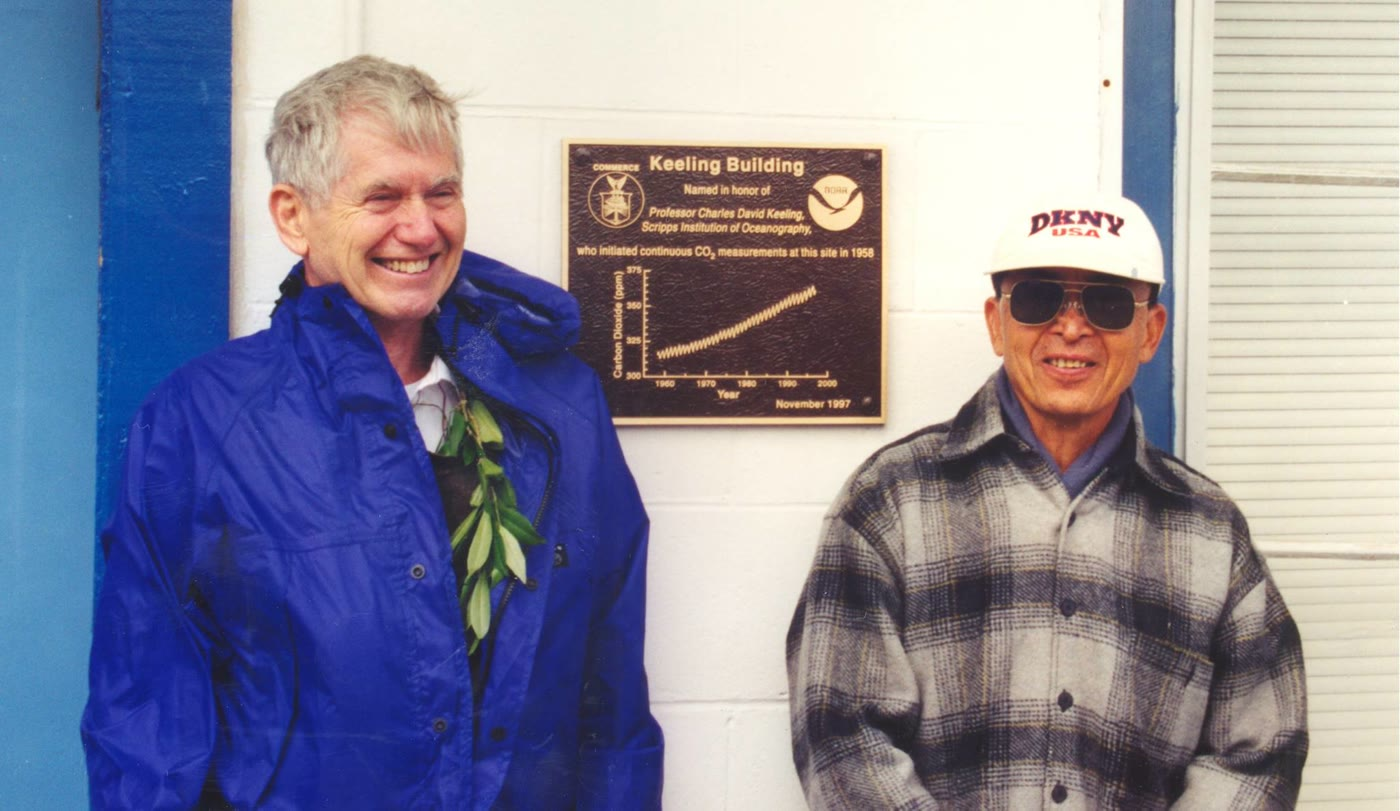
\includegraphics[width=0.62\linewidth]{images/book2/g12-noaa-keeling-chin-1997.jpg}

{\small Charles David Keeling (kiri) dan John Chin di Observatorium Mauna Loa
pada 1997, di samping plakat yang menamai sebuah gedung dengan nama Keeling.
Foto: John Miller, NOAA (domain publik).}
\end{center}
\end{history}

\section{Latihan}

\begin{exercise}[$\star$]\label{exo:g12:climate-change:1}
Apa \omterm{def:g12:climate-change:forcing}{gaya radiatif} sebuah perubahan dalam sistem iklim? Dalam satuan apa \omterm{def:g12:climate-change:forcing}{gaya}
itu diukur, dan apa arti tandanya?
\end{exercise}

\begin{exercise}[$\star$]\label{exo:g12:climate-change:2}
Pada bulan apa dalam setahun konsentrasi karbon dioksida di Mauna Loa paling
tinggi, dan pada bulan apa paling rendah? Jelaskan ayunan tahunan itu.
\end{exercise}

\begin{exercise}[$\star$]\label{exo:g12:climate-change:3}
Dalam kosakata penilaian, peluang berapa yang dimaksud dengan \emph{sangat
mungkin}? Dan \emph{mungkin}? Apa arti rentang yang ditulis
$[0.95 \text{ sampai } 1.20]$?
\end{exercise}

\begin{exercise}[$\star$]\label{exo:g12:climate-change:4}
Dari energi tambahan yang diperoleh sistem iklim dalam dekade-dekade terakhir,
berapa bagian yang masuk ke samudra? Mengapa hal ini menjelaskan bahwa
permukaan laut naik bahkan tanpa es yang mencair?
\end{exercise}

\begin{exercise}[$\star$]\label{exo:g12:climate-change:5}
Berikan dua \omterm{def:g12:climate-change:feedback}{umpan balik iklim} positif dan tanggapan negatif yang membatasi
pemanasan. Jelaskan masing-masing dalam satu kalimat.
\end{exercise}

\begin{exercise}[$\star\star$]\label{exo:g12:climate-change:6}
Konsentrasi karbon dioksida rata-rata tahunan di Mauna Loa adalah
\qty{315.98}{ppm} pada 1959 dan \qty{427.35}{ppm} pada 2025. Berapa ppm, dan
berapa persen, kenaikannya? Berapa pertambahan rata-rata per tahun selama
seluruh periode itu?
\end{exercise}

\begin{exercise}[$\star\star$]\label{exo:g12:climate-change:7}
Gunakan hukum logaritmik dalam bab ini, dengan $F_{2\times} =
\qty{3.93}{W/m^2}$ dan $C_0 = \qty{278}{ppm}$, untuk menghitung \omterm{def:g12:climate-change:forcing}{gaya} karbon
dioksida pada \qty{427.35}{ppm}, rata-rata tahunan 2025.
\end{exercise}

\begin{exercise}[$\star\star$]\label{exo:g12:climate-change:8}
Dengan laju \qty{3.7}{mm} per tahun, laju 2006--2018, berapa permukaan laut
akan naik dalam 30 tahun? Berapa kali lebih cepat laju ini daripada laju
1901--1971, \qty{1.3}{mm} per tahun?
\end{exercise}

\begin{exercise}[$\star\star$]\label{exo:g12:climate-change:9}
Dengan $\Delta T = F/\lambda$ dan $\lambda = \qty{1.16}{W.m^{-2}.\degreeCelsius^{-1}}$,
hitung pemanasan kesetimbangan yang akan dihasilkan oleh \omterm{def:g12:climate-change:forcing}{gaya} manusia total
pada 2019, \qty{2.72}{W/m^2}. Pemanasan yang teramati akibat manusia hanya
sekitar \qty{1.07}{\degreeCelsius}. Berikan alasan utama perbedaannya.
\end{exercise}

\begin{exercise}[$\star\star$]\label{exo:g12:climate-change:10}
Matahari dan gunung api mengubah suhu global antara 1850--1900 dan
2010--2019 sebesar $-0.1$ sampai $+\qty{0.1}{\degreeCelsius}$, sedangkan
pemanasan yang teramati sekitar \qty{1.06}{\degreeCelsius}. Apa kesimpulanmu?
Penyebab alami lain apa yang juga harus disingkirkan, dan apa kata penilaian
tentangnya?
\end{exercise}

\begin{exercise}[$\star\star$]\label{exo:g12:climate-change:11}
Dengan tabel \omterm{def:g12:climate-change:scenario}{proyeksi}, dalam \omterm{def:g12:climate-change:scenario}{skenario} mana pemanasan 2081--2100 sangat mungkin
tetap di bawah \qty{2}{\degreeCelsius}? Dalam \omterm{def:g12:climate-change:scenario}{skenario} mana pemanasan itu
sangat mungkin melampaui \qty{2}{\degreeCelsius}?
\end{exercise}

\begin{exercise}[$\star\star\star$]\label{exo:g12:climate-change:12}
Aerosol menghasilkan \omterm{def:g12:climate-change:forcing}{gaya} sekitar $-0.22$ dan $\qty{-0.84}{W/m^2}$
(melalui sinar Matahari dan melalui awan). Bila semua aerosol dihilangkan dari
udara sementara segala hal lain tetap seperti pada 2019, menjadi berapa \omterm{def:g12:climate-change:forcing}{gaya}
manusia total? Berapa pemanasan kesetimbangan akan bertambah, dengan
$\lambda = \qty{1.16}{W.m^{-2}.\degreeCelsius^{-1}}$?
\end{exercise}

\begin{exercise}[$\star\star\star$]\label{exo:g12:climate-change:13}
Tunjukkan, dari hukum logaritmik, bahwa kenaikan dari \qty{278}{ppm} ke
\qty{556}{ppm} dan kenaikan dari \qty{556}{ppm} ke \qty{1112}{ppm} menambahkan
\omterm{def:g12:climate-change:forcing}{gaya} yang sama. Berapa \omterm{def:g12:climate-change:forcing}{gaya} total pada \qty{1112}{ppm}?
\end{exercise}

\begin{exercise}[$\star\star\star$]\label{exo:g12:climate-change:14}
Turunkan hukum logaritmik terhadap $C$. Berapa \omterm{def:g12:climate-change:forcing}{gaya} yang ditambahkan satu ppm
karbon dioksida tambahan pada \qty{280}{ppm}, dan berapa pada
\qty{420}{ppm}? Berikan komentar.
\end{exercise}

\begin{exercise}[$\star\star\star$]\label{exo:g12:climate-change:15}
Tanpa \omterm{def:g12:climate-change:feedback}{umpan balik} apa pun kecuali radiasi tambahan ke angkasa,
$\lambda_0 = \qty{3.22}{W.m^{-2}.\degreeCelsius^{-1}}$. Hitung pemanasan
untuk penggandaan karbon dioksida ($F_{2\times} = \qty{3.93}{W/m^2}$) dengan
$\lambda_0$, lalu dengan $\lambda = \qty{1.16}{W.m^{-2}.\degreeCelsius^{-1}}$.
Dengan faktor berapa \omterm{def:g12:climate-change:feedback}{umpan balik} memperkuat pemanasan itu?
\end{exercise}

\section{Soal: Kurva Keeling dalam Angka}

\begin{problem}[{Soal akhir pekan --- dari napas tahunan vegetasi sampai
tahun tercapainya penggandaan}]
\label{pb:g12:climate-change:1}
% ledger: data:co2-mlo (annual means 1960 316.91, 1970 325.68, 2015 401.01,
% 2025 427.35; seasonal departures May +3.37, September -3.51, means of
% 2015-2024; all from figdata/grade-12/climate_records.py), noaa:mlo-site,
% ipcc:erf-2xco2, ipcc:ecs, ipcc:feedbacks, ipcc:co2-2myr
Seorang siswa mengunduh rekaman Mauna Loa dan mengolahnya dengan lembar kerja.
Selama 2015--2024, konsentrasi bulanan rata-rata terletak \qty{3.37}{ppm} di
atas tren yang dihaluskan pada bulan Mei dan \qty{3.51}{ppm} di bawahnya pada
bulan September. Rata-rata tahunannya \qty{316.91}{ppm} pada 1960,
\qty{325.68}{ppm} pada 1970, \qty{401.01}{ppm} pada 2015, dan \qty{427.35}{ppm}
pada 2025. Konsentrasi pada 1750 adalah \qty{278}{ppm}. Gunakan hukum
logaritmik dengan $F_{2\times} = \qty{3.93}{W/m^2}$.

\medskip
\noindent\textbf{Bagian I --- Napas vegetasi.}
\begin{enumerate}
  \item Berapa amplitudo puncak-ke-lembah siklus tahunan itu?
  \item Jelaskan mengapa konsentrasinya paling tinggi pada bulan Mei dan paling
        rendah pada bulan September.
  \item Siklus itu jauh lebih lemah di udara Belahan Bumi Selatan. Kemukakan
        alasannya.
  \item Mengapa observatorium itu dibangun setinggi \qty{3397}{m}, di atas
        sebuah gunung api di tengah Pasifik?
\end{enumerate}

\medskip
\noindent\textbf{Bagian II --- Trennya.}
\begin{enumerate}[resume]
  \item Hitung pertambahan rata-rata, dalam ppm per tahun, selama 1960--1970.
  \item Hitung pertambahan itu selama 2015--2025.
  \item Dengan faktor berapa laju pertambahan itu meningkat?
  \item Berapa persen konsentrasi itu naik antara 1750 dan 2025?
  \item \omterm{def:g12:past-climates:ice-core}{Inti es} tidak pernah menunjukkan lebih dari sekitar \qty{300}{ppm}
        selama 800\,000 tahun terakhir. Berapa ppm nilai 2025 melampauinya?
\end{enumerate}

\medskip
\noindent\textbf{Bagian III --- Gayanya.}
\begin{enumerate}[resume]
  \item Hitung \omterm{def:g12:climate-change:forcing}{gaya} karbon dioksida pada 2025.
  \item Hitung \omterm{def:g12:climate-change:forcing}{gaya} itu pada 1960, dan kenaikan \omterm{def:g12:climate-change:forcing}{gaya} antara 1960 dan 2025.
  \item Konsentrasi berapa yang akan menambahkan \qty{1}{W/m^2} pada \omterm{def:g12:climate-change:forcing}{gaya}
        tahun 2025?
  \item Dengan laju pertambahan 2015--2025, berapa tahun yang diperlukan untuk
        itu?
\end{enumerate}

\medskip
\noindent\textbf{Bagian IV --- Penggandaan.}
\begin{enumerate}[resume]
  \item Berapa konsentrasi penggandaan nilai tahun 1750? Berapa \omterm{def:g12:climate-change:forcing}{gaya} yang
        dihasilkannya?
  \item Dengan perkiraan terbaik \omterm{def:g12:climate-change:ecs}{sensitivitas iklim kesetimbangan}, berapa
        pemanasan kesetimbangan yang akan ditimbulkannya? Berikan rentang
        mungkinnya.
  \item Parameter \omterm{def:g12:climate-change:feedback}{umpan balik} $\lambda$ berapa yang tersirat dari sensitivitas
        \qty{3}{\degreeCelsius}? Bandingkan dengan nilai
        \qty{1.16}{W.m^{-2}.\degreeCelsius^{-1}} yang diperoleh dengan
        menjumlahkan \omterm{def:g12:climate-change:feedback}{umpan balik-umpan baliknya}.
  \item Mengapa permukaan tidak akan mencapai pemanasan ini pada hari
        penggandaan itu tercapai?
  \item Mengapa perhitungan yang sekadar memperpanjang laju pertambahan
        sekarang adalah sebuah \omterm{def:g12:climate-change:scenario}{skenario}, dan bukan \omterm{def:g12:climate-change:scenario}{proyeksi} seperti yang dibuat
        oleh penilaian-penilaian?
  \item Bila laju pertambahan 2015--2025 tetap sama, pada tahun berapa
        penggandaan konsentrasi tahun 1750 akan tercapai?
\end{enumerate}
\end{problem}
